\documentclass[xcolor=dvipsnames,table]{beamer}

\usepackage{latexsym}
\usepackage[utf8]{inputenc}
\usepackage[brazil]{babel}
\usepackage{amssymb}
\usepackage{amsmath}
\usepackage{stmaryrd}
\usepackage{fancybox}
\usepackage{datetime}
\usepackage[T1]{fontenc}
\usepackage{graphicx}
\usepackage{graphics}
\usepackage{url}
\usepackage{algorithmic}
\usepackage{algorithm}
\usepackage{acronym}
\usepackage{array}

\newtheorem{definicao}{Definio}
\newcommand{\tab}{\hspace*{2em}}

\mode<presentation>
{
  \definecolor{colortexto}{RGB}{0,0,0}
 
  \setbeamertemplate{background canvas}[vertical shading][ bottom=white!10,top=white!10]
  \setbeamercolor{normal text}{fg=colortexto} 

  \usetheme{Warsaw}
}

\title{Grafo Bipartido} 

\author{
  Esdras Lins Bispo Jr. \\ \url{bispojr@ufg.br}
  } 
 \institute{
  Teoria de Grafos \\Bacharelado em Ciência da Computação}
\date{\textbf{23 de maio de 2017} }

\logo{
\includegraphics[width=1cm]{images/ufgJataiLogo.png}}

\begin{document}

	\begin{frame}
		\titlepage
	\end{frame}

	\AtBeginSection{
		\begin{frame}{Sumário}%[allowframebreaks]{Sumário}
    		\tableofcontents[currentsection]
    		%\tableofcontents[currentsection, hideothersubsections]
		\end{frame}
	}

	\begin{frame}{Plano de Aula}
		\tableofcontents
		%\tableofcontents[hideallsubsections]
	\end{frame}
    
    \begin{frame}{Pensamento}
		\begin{columns}
			\column{.4\textwidth}  		
		  		\begin{center}
		    		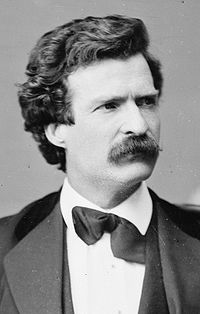
\includegraphics[height=.8\textheight]{images/mark.jpg}
		  		\end{center}
			\column{.6\textwidth}  		
				\begin{block}{Frase}
					\begin{center}
						{\large A gente não se liberta de um hábito atirando-o pela janela: é preciso fazê-lo descer a escada, degrau por degrau.}
					\end{center}
				\end{block}		  		
		  		\begin{block}{Quem?}
		  			\begin{center}
						{\bf Mark Twain (1835 - 1910)} \\Escritor e humorista estadunidense
					\end{center}
				\end{block}
		\end{columns}
	\end{frame}
    
    \section{Revisão}
	\subsection{Matriz de adjacências e incidências}
	\begin{frame}{Matriz de adjacências e incidências}
		\begin{block}{Definição}
			Uma {\bf matriz de adjacências} de um grafo $G$ é a matriz $A$ definida da seguinte maneira: para todo vértice $u$ e $v$
			\begin{center}
				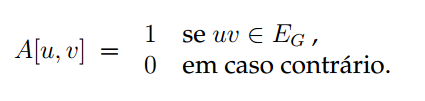
\includegraphics[width=.5\textwidth]{images/adjacencia.png}
			\end{center}
		\end{block} 
		\begin{block}{Definição}
			Uma {\bf matriz de incidências} de um grafo $G$ é a matriz $M$ definida da seguinte maneira: para todo vértice $u$ e uma aresta $e$
			\begin{center}
				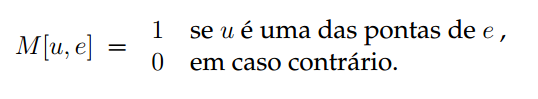
\includegraphics[width=.6\textwidth]{images/incidencia.png}
			\end{center}
		\end{block}
	\end{frame}

	\section{Grafos Bipartidos}
	\begin{frame}{Grafo Bipartido}
		\begin{block}{Definição}
			Um grafo $G$ é {\bf bipartido} se existe uma bipartição $\{U, W \}$ de $V_G$ tal que toda aresta de $G$ tem uma ponta em $U$ e outra em $W$.
		\end{block} \pause
		\begin{block}{Lembrando... Bipartição!}
			Uma bipartição de um conjunto $V$ é um par $\{U, W\}$ de conjuntos não vazios tal que $U \cup W = V$ e $U \cap W = \emptyset$.
		\end{block} \pause
		\begin{block}{Notação}
			\begin{itemize}
				\item Para explicitar a partição, podemos dizer que o grafo é {\bf $\{ U, W \}$-bipartido}. \pause
				\item Se $G$ é um grafo $\{ U, W \}$-bipartido, podemos dizer, informalmente, que os elementos de $U$ são os {\bf vértices brancos} e os de $W$ são os {\bf vértices pretos} do grafo.
			\end{itemize}
		\end{block} 
	\end{frame}
	
	\begin{frame}{Grafo Bipartido}
		\begin{block}{Grafo $\{ U, W \}$-bipartido completo}
			Um grafo $\{U, W \}$-bipartido é {\bf completo} se todo vértice branco é adjacente a todos os vértices pretos. 
		\end{block} \pause
		\begin{center}
			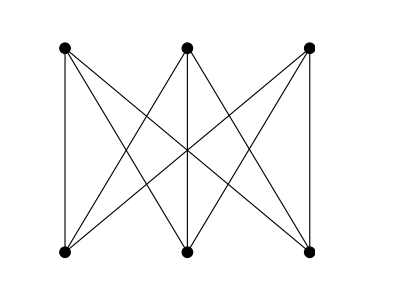
\includegraphics[width=.6\textwidth]{images/bipartido-completo.png}
		\end{center}
	\end{frame}
	
	\begin{frame}{Grafo Bipartido}
		\begin{block}{$K_{p,q}$}
			Um $K_{p,q}$ é um grafo bipartido completo com \\$p$ vértices brancos e $q$ pretos.
		\end{block} \pause
		\begin{block}{Estrela}
			\begin{itemize}
				\item Uma {\bf estrela} é um grafo $K_{1,q}$; \pause
				\item Se $q \geq 2$, o {\bf centro} da estrela é o único vértice que incide em duas ou mais arestas; \pause
				\item Se $q < 2$, a estrela não tem centro.
			\end{itemize}
		\end{block}
	\end{frame}
	
	\begin{frame}
		\titlepage
	\end{frame}
	
\end{document}